\documentclass[a4paper,12pt]{article}
\usepackage{amsmath,amsfonts,amsthm,amscd,amssymb,latexsym,eufrak}
%%%%%%%%%%%%%
\usepackage{enumerate,graphicx,psfrag,subfigure}%,jchangebar,oldgerm}
\usepackage[mathscr]{eucal}
\usepackage[usenames]{color}
\usepackage{url}
%\usepackage{showkeys}
%%%%%%%%%
\sloppy

%%\documentclass[12]{article}


%%%%%%%%%%%%%%%%%%%%%%%
%
%
%
\title{The subgroup membership problem
}
\author{Andrew J. Duncan, Elizaveta Frenkel}

%%%%%%%%%%%Liza to compile
%\newtheorem{theorem}{Theorem}[section]
%\newtheorem{maintheorem}{Theorem}[]
%\newtheorem{lemma}[theorem]{Lemma}
%\theoremstyle{definition}
%\newtheorem{algorithm}[theorem]{Algorithm}
%\newtheorem{corollary}[theorem]{Corollary}
%\newtheorem{conjecture}[theorem]{Conjecture}
%\newtheorem{definition}[theorem]{Definition}
%\newtheorem{example}[theorem]{Example}
%\newtheorem{problem}[theorem]{Problem}
%\newtheorem{question}[theorem]{Question}
%\newtheorem{remark}[theorem]{Remark}
%\newtheorem{proposition}[theorem]{Proposition}
%\newtheorem{convention}[theorem]{Convention}
%\newtheorem{comment}[theorem]{Comment}
%\newtheorem{claim}[theorem]{Claim}
%%\newtheorem{procedure}{Procedure}%[theorem]%[section]
%\newtheorem{procedure}{Procedure}[section]%[theorem]
%%%\newtheorem{proof}[proof]{Proof}
%%%%%%%%%%%Liza to compile



%%%%%%%%%%%%%%%%%%%%%%%%%%%
%%%%%%%%%%%%%%%%%%%%%%%%%%%
\renewcommand{\a}{\alpha }
\renewcommand{\b}{\beta }
\newcommand{\G}{\Gamma }
\newcommand{\g}{\gamma }
\newcommand{\D}{\Delta }
\renewcommand{\d}{\delta }
%\def\vd{\vardelta}
\newcommand{\ep}{\epsilon }
\newcommand{\e}{\varepsilon }
\newcommand{\z}{\zeta }
%\eta
\renewcommand{\th}{\theta }
\newcommand{\T}{\Theta }
\renewcommand{\i}{\iota }
\renewcommand{\k}{\kappa }
\renewcommand{\l}{\lambda }
\renewcommand{\L}{\Lambda }
%\mu
%\nu
%\xi
%omicron
%\pi
\renewcommand{\r}{\rho }
\newcommand{\s}{\sigma }
\renewcommand{\S}{\Sigma }
\renewcommand{\t}{\tau }
\newcommand{\up}{\upsilon }
\newcommand{\U}{\Upsilon }
%\phi
\newcommand{\x}{\chi }
%\psi
\newcommand{\W}{\Omega }
\newcommand{\w}{\omega }
%%%%%%%%%%%%%%%%%%%%%%%%%%%%%%%
%%%%%%%%%%%%%%%%%%%%%%%%%%%%%
\newcommand{\pd}{\partial}
\newcommand{\wht}{\widehat}
%\newcommand{\cC}{{\mathcal C}}
%\newcommand{\cdim}{\texttt{cdim}}
\newcommand{\fC}{{\textswab C}}
\newenvironment{ef}{\noindent\color{blue} \bf EF: }{}
%
\newcommand{\cA}{{\cal{A}}}
\newcommand{\cD}{{\cal{D}}}
\newcommand{\cF}{{\cal{F}}}
\newcommand{\cH}{{\cal{H}}}
\newcommand{\cJ}{{\cal{J}}}

\newcommand{\cK}{{\cal{K}}}
\newcommand{\cP}{{\cal{P}}}
\newcommand{\cR}{{\cal{R}}}
\newcommand{\cS}{{\cal{S}}}
\newcommand{\cW}{{\cal{W}}}
\newcommand{\cQ}{{\cal{Q}}}
%\newcommand{\GG}{\ensuremath{\mathbb{G}}}
\newcommand{\pp}{\mathbf{p}}
%%%%%%%%%%%%%%%%%%%%%%%%%%%%%%
\newcommand{\nul}{\emptyset }

%%%%%%%%%%%%%%%%%%%%%%%%%%%%%%
\newtheorem{theorem}{Theorem}[section]
\newtheorem{lemma}[theorem]{Lemma}
\newtheorem{corollary}[theorem]{Corollary}
\newtheorem{proposition}[theorem]{Proposition}
\newtheorem{axiom}[theorem]{Axiom}
\newtheorem{definition}[theorem]{Definition}
\newtheorem*{defn*}{Definition}
\newtheorem{conjecture}[theorem]{Conjecture}
%cvs -d :pserver:najd2@cvs.mas.ncl.ac.uk:/CVS/najd2
\newtheorem{exam}[theorem]{Example}
\newtheorem{comment}[theorem]{Comment}
%
%
\newenvironment{example}{\begin{exam} \rm}{\end{exam}}
%
%
%
\newtheorem{remk}[theorem]{Remark}
\newenvironment{remark}{\begin{remk} \rm}{\end{remk}}
%
%%%%%%%%%%%%
\numberwithin{equation}{section}
\numberwithin{figure}{section}
%%%%%%%%%%%%%%%%%%%%
\newcommand{\Iso}{\operatorname{Isom}}
\newcommand{\Aut}{\operatorname{Aut}}
%%%%%%%%%%%%%%%%%%%
\renewcommand{\AA}{\ensuremath{\mathbb{A}}}
\newcommand{\ZZ}{\ensuremath{\mathbb{Z}}}
\newcommand{\QQ}{\ensuremath{\mathbb{Q}}}
\newcommand{\RR}{\ensuremath{\mathbb{R}}}
\newcommand{\NN}{\ensuremath{\mathbb{N}}}
\newcommand{\CC}{\ensuremath{\mathbb{C}}}
\newcommand{\FF}{\ensuremath{\mathbb{F}}}
%\renewcommand{\ker}{\verb"Ker"}
\newcommand{\cC}{\mathcal{C}}
\newcommand{\cO}{\mathcal{O}}
\newcommand{\la}{\langle}
\newcommand{\ra}{\rangle}
%\newcommand{\BA}{\ensuremath{\mathbb{A}}}
%%%%%%%%%%%%%%%%%%%%%%%%%%%%%%%%%%%%%%
\newcommand{\maps}{\rightarrow}
\newcommand{\ov}[1]{\overline{#1}}
\newcommand{\bs}{\backslash}
%%%%%%%%%%%%%%%%%%%%%%%%%%%%%%%
\newcommand{\be}{\begin{enumerate}}
\newcommand{\ee}{\end{enumerate}}
\newcommand{\bd}{\begin{description}}
\newcommand{\ed}{\end{description}}
%%%%%%%%%%%%%%%%%%%%%%%%%%%%%%%%%%%
%
\newenvironment{ajd}{\noindent\color{blue} AJD }{}
\newenvironment{xxx}{\noindent\color{red}}{}
%
\begin{document}
\maketitle

\begin{abstract}
We modify Stallings folding theory to apply it to amalgamated
products of finite rank free groups. Using special kind of normal
forms, we show how they can be used to decide subgroup membership
problem for free products with amalgamation.
 \end{abstract}



\section{Introduction}\label{se:global_intro}
Stallings introduced his technique of foldings in his paper
\cite{stallings83} where he applied this technique to investigate
free groups. In his \cite{stallings88} Stallings extend ideas of
foldings to non-free actions of groups on graphs and trees. Next
years ideas of Stallings was widely generalized in different
directions and applied to decide different problems in
combinatorial group theory, see for example
\cite{befe,BoWei,KM02,SilvaWeil08}.

Let $G = <X|R>$ be a finitely generated group. The group $G$ has
solvable membership problem if there is an algorithm which, for
any finite set of words $w, k_1, \ldots k_s$ in $G$ decides
whether or not the element $w$ belongs to the subgroup $K = <k_1,
\ldots, k_s>$. In this paper we decide the subgroup membership
problem for amalgamated products of finite rank free groups, using
a language of special normal forms for elements of such groups and
extending ideas of Stallings foldings for this group construction.
Free group constructions, in particular, free products of groups,
with or without amalgamation, $HNN-$extensions
 and, more generally, fundamental groups
of graphs of groups represent a subject of special interest in
group theory from different points of view. First results here
related to the solvability of membership problem in group
constructions described above is due to Mihailova (see
\cite{mi59,mi68}), who shown that the membership problem is
decidable in free product of groups $A$ and $B$ if it is decidable
in both factors. One should mention also another famous result of
Mihailova \cite{mi58} which provide an important counter-example
in this direction. Namely, she constructed a finitely generated
subgroup of direct product of two free groups of rank two with
unsolvable membership problem; notice also, that this direct
product can be considered also as sequence of two $HNN-$extensions
of rank two free group. On the other hand, it is another classical
result that a free group of finite rank has solvable (uniform)
membership problem. It shows, that even innocent group
constructions can affect solvability of the membership problem
dramatically.

The membership problem for free products with amalgamation and
$HNN-$extension was studied by Bezverkhnii in his papers
\cite{bez81,bez86,bez90,bez91}, where he used combinatorial
technique and standard normal forms in amalgamated product of
groups. Our approach is, first of all, more geometrical, and since
we have an eye on generalization of this result on other free
constructions, we were obliged to introduce another language to
study these constructions. Another significant step in this
direction was done by Kapovich, Miasnikov and Weidmann in their
paper \cite{KMW03}, where authors investigated uniform membership
problem for fundamental groups of graph of groups under certain
assumptions on both vertices and edges groups. In particular, they
shown that for the case where all vertices groups either locally
quasiconvex wordhyperbolic or polycyclic-by-finite and all edges
groups are polycyclic-by-finite the uniform membership problem for
fundamental groups of such a graph of groups is solvable.

As it was mentioned above, we want to introduce geometric
technique, which relies on Stallings foldings ideas and another
type of normal forms for elements of amalgamated products of
groups. Now, a few words on the structure of the paper. In Section
\ref{sec:intro} we introduce the double coset normal forms for
elements amalgamated products of finite rank free groups.
 In Section \ref{sec:dcforms} we study the structure of these double coset normal forms and describe the explicit procedure
 of their construction. Namely, we show how to obtain a unique normal form of an element in a free group of finite
 rank; these forms are based on double coset of representatives of
 two types representatives (see subsection \ref{sub:2cosetrepr}).
 Simple procedure described in the beginning of \ref{sec:foldings}
 shows how to rewrite arbitrary word in a reduced form into double
 coset normal form using these special representations in factors.

Section  \ref{sec:foldings} is the heart of the paper. Let $K$ be
a subgroup of an amalgamated product of finite rank free groups.
Using the notion of double coset graph (automaton), we extend
folding procedure such the after the sequence of transformations
of double coset graph for $K$ the resulting graph recognize
precisely normal forms of elements of $K$.



Authors are grateful to Vladimir Remeslennikov for helpful
discussions and to Christian Perfect who did something.{\ef Should
we mention VNR here or among the authors? What should we say about
Christian's work?}



\section{Double coset normal form}\label{sec:intro}
Based on notes copied (laboriously) from Christian's page
\url{
http://checkmyworking.com/misc/writemaths/?doublecoset
}

$F_1$, $F_2$ free groups (finitely generated by $X_1$
and $X_2$, respectively).

Let $H_1 \leq F_1$, $H_2 \leq F_2$ such that
there exists an isomorphism $\phi: H_1 \rightarrow H_2$.

i.e. we have finite bases $\{h_1, \ldots, h_m \}$  for $H_1$ and
$\{h_1', \ldots, h_m'\}$ for $H_2$.

Consider the free group $F(Z)$, generated by $Z=\{z_1, \ldots, z_m\}$,
and the maps $\phi_1$ and $\phi_2$ such that
$\phi_1(z_i)=h_i(X_1)  $ and  $\phi_2(z_i)=h^\prime_i(X_2)$, $i=1,\ldots ,m$.
Thus $\phi_i$ extends to an isomorphism of $F(Z)$ to $H_i$. We choose
the $\phi_i$ so that $\phi=\phi_2\phi_1^{-1}$.

Let ${G = F_1 \underset{H_1=H_2}{\ast} F_2}$, the group with
 presentation \[\la X_1,X_2 | h_i = h_i', i=1, \ldots ,m\ra.\]

A  set $S_i \subseteq F_i$ such that
\be
\item
$F_i = \displaystyle{\bigcup_{s \in S_i} H_isH_i}$
and
\item
for all $s, s^\prime \in S_i$, $s\in H_i s^\prime H_i$
implies $s=s^\prime$,
\ee
is called a set of \emph{double coset representatives for} $H_i\le F_i$.

Let $S_1$ and $S_2$ be sets of  double coset representatives of
$H_1\le F_1$ and $H_2\le F_2$, respectively. Let $g \in G$.
A word $w$ representing $g$ is in \emph{(double coset) normal form} if
$w = h_{0}p_1h_{1}p_2 \cdots h_{k-1}p_kh_{{k}}$, $k\ge 0$,  with
\be
\item $p_i \in S_1\cup S_2$  and $h_i$ is a reduced word in $F(Z)$ and
\item if $p_i\in S_j$ then $p_{i+1}\notin S_j$, for $j=1$ and $2$,
\ee
for $i = 1, \ldots ,k$.


\section{Constructing double coset representatives}\label{sec:dcforms}

Given an arbitrary word $g\in F_1\ast F_2$,
we should like an algorithm to write $g$ in double coset normal form
with respect to some choice of double coset representatives. We may
assume (after free cancellation if necessary) that $g$ is a
reduced word in $((X_1\cup X_2)\cup ( X_1^{-1}\cup X_2^{-1}))^\ast$.

First we say $g$ is in \emph{reduced form} if $g = g_1 \cdots g_t$, where
$g_1 \in F_1$ or $g_1 \in F_2$ and
for
$i > 1$,    $g_i \in (F_1 \backslash H_1)\cup (F_2\backslash H_2)$ and  $g_i$
and  ${g_{i+1}}$ belong to  different factors. As $F_1$ and
$F_2$ have solvable subgroup membership problem we can write $g$ in
reduced form. More precisely, we construct a Stallings automaton
(see below) $A_k$ for
$H_k\le F_k$. % and choose a maximal subtree $T_k$ of $A_k$, $k=1,2$.
Then we write $g=f_1\cdots f_r$, in free product normal
form (each $f_i$ is in a factor and successive terms are
from different factors).
Now,
using the appropriate Stallings automaton $A_k$, we write $f_r=h_rg_r$, where
$h_r$ is the maximal prefix of $f_r$ accepted by $A_k$ and $g_r$ is
 the
unique word such that $f_r=h_rg_r$, reduced as written.

Using the maps $\phi_1$ and $\phi_2$ we now write $h_r$ in terms of the
generators of the other factor, to obtain $h^\prime_r$ and then
replace $f_{r-1}$ with $f_{r-1}^\prime=f_{r-1}h^\prime_r$. Now start again with
$f_{r-1}^\prime$ instead of $f_r$. Continue till the word is exhausted.
This gives $g=g_1\cdots g_t$ in reduced form.

To rewrite in double coset normal form we need to
 rewrite
each $g_i$ in double coset normal form in its factor,
with respect to some (fixed) set
of double coset representatives.

\subsection{Double coset representatives}\label{sub:2cosetrepr}
%{\bf We should include a short description of Stallings folding, as in
%Enric's notes from Manresa \cite{ventura11}.} \\[1em]

An {\em automaton} $A$ is  a quintuple
$(\S,Q,\d,\mathcal{S},\mathcal{F})$, where $\S$ is finite set
called the {\em alphabet}, $Q$ is a finite set of {\em states},
$\d$ is a map $\d:Q\times \S\maps Q$, called the {\em transition
function}, $\mathcal{S}\subset Q$ is the (non-empty) set of {\em
start states} and $\mathcal{F}\subseteq Q$ is the set of {\em
final states}. (Usually $\mathcal{S}$ is a singleton.) If
$\mathcal{F}=\{s_0\}=\mathcal{S}$ it's common to drop
$\mathcal{F}$ from the description and define $A$ as a quadruple.
The language accepted by an automaton $A$ (with any choice of
start state in $\mathcal{S}$) is denoted $L(A)$. If $\S$ is a
subset of a group $G$
 then the  natural map from $L(A)$ to
$G$ is denoted $\pi:L(A)\maps G$.

An automaton $A = (\S, Q, \d, \mathcal{S},\mathcal{F})$ is {\em
inversive} if $\S$ is an inversive alphabet and for all $p, q \in
Q$ and $a \in \S$ $\d(p,a)=q$ if and only if $\d(q, a^{-1})=p$.
Further, an automaton $A= (\S, Q, \d, s_0)$ is called {\em trim}
if it has no vertices of degree $1$ except maybe the basepoint
$s_0$. An automaton $A$ is {\em deterministic} if $\d(p,a)=q$ and
$\d(p,a)=q'$ imply $q=q'$.

 We shall associate to an automaton $A$
a directed, edge labelled graph $\G_A$ with vertices
$V=V(\G_A)=Q$; edge set $E=E(\G_A)$ consisting of elements
$(u,\s,v)$ of $Q\times \S\times Q$ such that $\d(u,\s)=v$; and
labelling function $l:E\maps \S$ given by $l(u,\s,v)=\s$, for all
$(u,\s,v) \in E$.  If $\mathcal{S}$ and $\mathcal{F}$ are the sets
of start and final states of $A$ we sometimes write
$(\G_A,\mathcal{S},\mathcal{F})$, and in particular if
$\mathcal{S}=\{s_0\}$ and $\mathcal{F}=\{f_0\}$, we write
$(\G_A,s_0,f_0)$ and if $S=\{s_0\}$ we call $s_0$ the {\em root}
vertex of $\G_A$. We say that graph $\G_A$ is {\em rooted} if
$s_0=f_0$, and we write $(\G_A,s_0)$ if this is the case. The
label $l(p)$ of a path is the concatenation of the labels of the
edge sequence of $p$. For notational simplicity we identify $\G_A$
and $A$ whenever it is convenient.

An automaton $A = (\G_A, \mathcal{S}, \mathcal{F})$ is {\em
inversive} if $\S$ is an inversive alphabet and $(u, \s, v) \in E
\Leftrightarrow (v, (\s)^{-1}, u) \in E$. From now we will
consider inversive automaton only. An automaton $A  = (\G_A,
\mathcal{S}, \mathcal{F})$ is {\em deterministic} if $(u, \s, v)
\in E$ and $(u, \s, v^\prime) \in E$ imply $v=v^\prime$. A rooted
automaton $A= (\G_A, s_0)$ is called {\em trim} if it has no
vertices of degree $1$ except maybe $s_0$.

Since we identify an automaton $A$ and graph $\G_A$, we ascribe
properties of $A$ to $\G_A$ (like trim, inversive or
deterministic) with exception that we use the term ``folded''
instead of ``deterministic'', for graphs.

%%Let $A=(V,E,s_0)$ and $A^\prime=(V^\prime,E^\prime,s^\prime_0)$ be
%%two automata. A {\em morphism} $A \rightarrow A^\prime$ is a map
%%$\varphi: V \rightarrow V^\prime$ such that $\varphi(s_0) =
%%s^\prime_0$ and $(p,a,q) \in E \Rightarrow
%%(\varphi(p),a,\varphi(q)) \in E^\prime$.
Recall the notion of standard Stalling foldings of automata, which
we will use directly for preparatory ``cleancing'' of an automaton
we will construct below, and in generalized form to produce
dc-foldings of this automaton (see Section \ref{sec:foldings}).

An {\em elementary folding} of a rooted graph $(\G_A,s_0)$ is a
graph $(\G^\prime_A,s^\prime_0)$ obtained from $(\G_A,s_0)$ as
follows. Suppose that $e=(u, \s, v)$ and $e^\prime=(u, \s,
v^\prime)$ are edges of $\G$. (We do not require $u$, $v$ and
$v^\prime$ to be distinct.)
 Then $\G^\prime_A$ is the quotient of $\G_A$ formed by identifying
$v$ and $v^\prime$, to form a new vertex $v^{\prime\prime}$; and
$e$ and $e^\prime$, to form a new edge $e^{\prime\prime}=(u, \s,
v^{\prime\prime})$. If $s_0= v$ or $s_0 = v^\prime$ then
$v^{\prime\prime}$ is the root of $\G^\prime$ and otherwise
$s^\prime_0=s_0$.
 A {\em folding} of a graph $\G$ is a graph obtained
from $\G$ by a finite sequence of elementary foldings.


Let $X$ be a finite alphabet, $F=\FF(X)$ and $H$ a finitely generated subgroup
of $F$.  By a {\em reduced} word we mean
 a freely reduced word in $(X\cup X^{-1})^\ast$, and we write $w\in F(X)$
to mean that $w$ is a reduced word. For $u,v, w\in F(X)$ we
write $w=u\circ v$ if $|w|=|u|+|v|$, in which case we say that $u$ is a {\em prefix}
of $w$.

Let $A$ be the Stallings automaton for $H$. Fix a spanning tree
$T$ for $A$. For each vertex $v$ of $A$ let $w(v)$ denote the
label of the path from $s_0=1$ to $v$ in $T$. We say the word $w$
is {\em readable} by $A$ if, starting in the start state $1$ with
input $w$, the automaton finishes with the empty word in some
arbitrary state. If $w$ is readable by $A$ we denote the final
state of $A$ after reading $w$ (starting in state $1$) by $\t(w)$.
If $w$ is readable by $A$ and $\t(w)=1$
 then we say $w$ is {\em accepted} by $A$. Define
\[L_T=\{w(v): v \textrm{ is a vertex of } A\}.\]
If $w, s\in F(X)$ then we say that $s$ is a {\em maximal}
$L_T${\em -prefix} of $w$ if $s\in L_T$, $w=s\circ u$ and no
longer prefix of $w$ belongs to $L_T$.

We shall define a set of double coset representatives for $H$ in two parts.
First, a word $w\in F(X)$ is a {\em representative of type} $1$ if
\[w=s\circ e \circ t^{-1},\]
where $s$ is a maximal $L_T$-prefix of $w$, $t$ is a maximal
$L_T$-prefix of $t\circ e^{-1}$ and $e\neq 1$.
\begin{comment} Notions of $L_T$-prefixes, maximal prefixes etc are closely related to the theory of (usual) coset
 representatives and there is a lot of things known about them (one-to-one correspondence between them and spanning subtrees etc. etc).
 We don't need to replace this definition since it looks convenient and compact, but, probably, we should refer reader to it... what do you think?
\end{comment}


Let $S^{(1)}$ denote the set of all representatives of type $1$.

To describe the remaining representatives we shall first define an equivalence
relation on the ordered pairs of distinct vertices of $A$. Let
\[P=\{(u,v)\in V(A)\times V(A): u\neq v\}.\]
Define a relation $\sim$ on $P$ by $(u_0,u_1)\sim (v_0,v_1)$ if and only if
there exist paths $p_0$ and $p_1$ in $A$, from $u_0$ to $v_0$ and $u_1$ to $v_1$
respectively, such that $l(p_0)=l(p_1)$. (We allow these paths to have length $0$.)
It is easy to verify that $\sim$ is an equivalence relation on $P$.

\begin{lemma}\label{lem:equiv_verts}
Let $(u_0,u_1)$ and $(v_0,v_1)$ be elements of $P$ and let
$a_0=w(u_0)$, $a_1=w(u_1)$, $b_0=w(v_0)$ and $b_1=w(v_1)$. Then
$(u_0,u_1)\sim (v_0,v_1)$ if and only if there exist $h_0,h_1\in H$ such that
\[a_0a_1^{-1}=h_0b_0b_1^{-1}h_1^{-1}.\]
\end{lemma}
\begin{proof}
$\Rightarrow$: Let $p_0$ and $p_1$ be paths, from $u_0$ to $v_0$ and $u_1$ to $v_1$
respectively, such that $l(p_0)=l(p_1)=c$, say. Set $h_0=a_0cb_0^{-1}$ and
$h_1=a_1cb_1^{-1}$. Since $h_0$ and $h_1$ are labels of closed paths in $A$, based at $1$, we
have $h_0$ and $h_1$ in $H$. Thus
$a_0a_1^{-1}=h_0b_0c^{-1}cb_1^{-1}h_1^{-1}=h_0b_0b_1^{-1}h_1^{-1}$, as required.

$\Leftarrow$: Let $h_0$, $h_1 \in H$ such that $a_0a_1^{-1}=h_0b_0b_1^{-1}h_1^{-1}$.
Set $k=a_0^{-1}h_0b_0=a_1^{-1}h_1b_1$. Then $h_0=a_0kb_0^{-1}$ and $h_1=a_1kb_1^{-1}$
belong to $H$ so there exist paths $p_0$ and $p_1$ in $A$,
from $\t(a_0)=u_0$ to $\t(b_0)=v_0$ and
$\t(a_1)=u_1$ to $\t(b_1)=v_1$, both with labels $k$.
Therefore $(u_0,u_1)\sim (v_0,v_1)$.
\end{proof}
\begin{comment}
It seems like we should specify different cases , depending on
$u_0, v_0$ and $u_1,v_1$ belonging to the same loop $h_i$ or not;
or something like this. Take an equivalence class as in example
\ref{ex:f_1f_2}. Then $a_0 = y_2^{-1}y_1$, $a_1 = y_1^2$, $b_0 =
y_2^{-1}$, $b_1=y_1$. Further, we obtain $c = y_1$ and the
equality satisfies, but with elements $h_0 = y_2^{-1} y_1^2 y_2$
and $h_1 = y_1^2$ which are not in $H_2$, as far as I understand.
Am I right or I misunderstood something?
\end{comment}

We shall choose one double coset representative corresponding to each $\sim$
equivalence class. To be explicit we make a particular choice of transversal
for the equivalence classes, as follows.
If $(u,v)\in P$ and $w(u)=a\circ x$, $w(v)=b\circ x$, for some $a,b\in F(X)$ and
$x\in X^{\pm 1}$, then $(\t(a),\t(b))\in P$ and $(u,v)\sim (\t(a),\t(b))$. It follows
that every equivalence class of $\sim$ contains an element $(a,b)$ such that
$w(a)w(b)^{-1}$ is a reduced word. Let $\pp$ be an equivalence class of $\sim$ and
let $Y$ be the set of all pairs $(u,v)\in \pp$ such that $|w(v)|$ is minimal (amongst
elements of $\pp$). Choose $(u,v)\in Y$ such that $|w(u)|$ is minimal (amongst elements
of $Y$) and define $(u,v)$ to be the $\sim${\em representative} of $\pp$. Fix
one $\sim$ representative for each equivalence class of $\sim$ and
let $Q$ denote the set of  all these $\sim$ representatives. A word $w\in F(X)$ is
 a {\em representative of type} $2$ if $w=w(u)w(v)^{-1}$, for some $(u,v)\in Q$.
Let $S^{(2)}$ denote the set of all representatives of type $2$
and define $S_1=S^{(1)}\cup S^{(2)}$. (Note that by the minimality
conditions of the definition, if $(u,v)$ is a $\sim$
representative then $w(u)w(v)^{-1}=w(u)\circ w(v)^{-1}$.) In order
to ensure uniqueness of the normal form of an element of $F(X)$ we
also need to choose an element $c(u,v)$ of $F(X)$, for each
$(u,v)\in P$, of $P$: $c(u,v)$ is defined to be the label of some
fixed choice of path from $u$ to $u_0$ and $v$ to $v_0$, where
$(u_0,v_0)$ is the $\sim$ representative of $(u,v)$.

\begin{proposition}\label{prop:dcreps}
$S_1$ is a set of double coset representatives for $H$.
\end{proposition}
\begin{proof}
First we shall show that every element $w\in F(X)$ lies in $HdH$,
for some $d\in S_1$. In fact we describe an algorithm which
rewrites a given word $w$ in this form.

Assume that the Stallings automaton $A$ for $H$ has been constructed by folding from
given generators for $H$. A spanning tree $T$
for $A$ may then be chosen and the
set $L_T$ computed. For each pair $(u,v)\in P$ the equivalence class $\pp$ of
$(u,v)$ may be constructed by considering all simple paths (no repeated vertices)
starting at $u$. A pair $(u^\prime ,v^\prime) \in P$ belongs to $\pp$
if and only
if there is a simple path from $u$ to $u^\prime$ with label $l$,
and a path from $v$ to $v^\prime$, also with label $l$.
Having constructed the equivalence classes of $\sim$
 a set of $\sim$ representatives may be constructed, by considering the
lengths of $w(a)$ and $w(b)$ for all $(a,b)$ in an equivalence class. Thus the
sets $Q$ and $S^{(2)}$ may be computed.   \\

\noindent{\bf The algorithm I}:\\
Input $w\in F(X)$.
Let $h$ be the maximal prefix of $w$ accepted by $A$; so $h\in H$ and
$w=h\circ f$, for some $f\in F(X)$. Now use $A$ to find the maximal prefix $p$
of $f$ which is readable by $A$;
 so $f= p\circ q$, for some $q\in F(X)$.

Next find the maximal prefix $g$ of $q^{-1}$ acceptable by $A$: say
$q^{-1}=g\circ r$, for some $r\in F(X)$, and then the maximal prefix
$t$ of $r$ which
is readable by $A$; say $r=t\circ e^{-1}$, for some $e\in F(X)$.

If $e\neq 1$ then
\[w=h\circ p \circ e\circ t^{-1}\circ g^{-1},\]
with $h,g\in H$. In this case $p$ and $t$ are readable by $A$. Set $y=w(\t(p))$
and $z=w(\t(t))$. Then $py^{-1}$ and $tz^{-1}$ belong to $H$. Moreover, as $p$
is the maximal prefix of $f$ readable by $A$  it is also the maximal
prefix of $pet^{-1}$ readable by $A$,  and so
  the
first letter of $e$ is not readable from the vertex $\t(p)=\t(y)$ of $A$.
In particular
$ye=y\circ e$. Similarly, the first letter of $e^{-1}$ is not readable from
the vertex $\t(t)=\t(z)$, so $ez^{-1}=e\circ z^{-1}$. Moreover $y$ is a
maximal $L_T$-prefix of $yez^{-1}$ and $z$ is a maximal $L_T$-prefix of $ze^{-1}$.
Thus $yez^{-1}\in S^{(1)}$ and we output
\[w=(py^{-1}) (yez^{-1})(zt^{-1})\in HS_1H,\]
of the required form.

On the other hand if $e=1$ then
\[w=h\circ p\circ t^{-1}\circ g.\]
In this case let $u=\t(p)$ and $v=\t(t)$,
let $(u_0,v_0)$ be the $\sim$ representative
of the equivalence class of $(u,v)$ and let $c=c(u,v)$.
Let $y=w(u_0)$ and $z=w(v_0)$. Then,  as in the proof of Lemma
\ref{lem:equiv_verts}, setting $h_0=w(u)c^{-1}y^{-1}$ and
$h_1=w(v)c^{-1}z^{-1}$ we have
 $h_0,h_1\in H$ and
\[w(u)w(v)^{-1}=h_0yz^{-1}h_1^{-1}.\] Furthermore
 $p w(u)^{-1}$ and  $t w(v)^{-1}$ are in $H$. Hence
\[
p\circ t^{-1}=( p w(u)^{-1})w(u)w(v)^{-1}( w(v)t^{-1})=( p w(u)^{-1}) h_0 yz^{-1}
h_1^{-1}( w(v)t^{-1})
\]
and by definition $yz^{-1}\in S^{(2)}$. We then output
\[w=a yz^{-1} b,\]
where $a=h ( p w(u)^{-1}) h_0\in H$ and $b=h_1^{-1}( w(v)t^{-1})g \in H$.

It remains to show that if $s_0,s_1\in S_1$ with $s_1\in Hs_0H$
then $s_1=s_0$. Suppose that $s_1=as_0b$, where $a, b\in H$. If
$s_0\in S^{(1)}$, say $s_0=y_0e_0z_0^{-1}$, then, as $ay_0$ and
$b^{-1}z_0$ are readable by $A$ and $e_0\neq 1$, it follows (as
above) that $s_1$ cannot be factored as $s_1=yz^{-1}$, where both
$y$ and $z$ are readable by $A$. Hence both $s_0$ and $s_1$ belong
to $S^{(1)}$ or both belong to $S^{(2)}$.

Consider the case where both belong to $S^{(1)}$ and, in the usual notation,
$s_i=y_i e_i z_i^{-1}$, $i=0,1$. We have $s_1=as_0b$, $a,b\in H$, and as $y_0$ has
no left divisor in $H$, if $a\neq 1$ then $a$ does not cancel completely with
 a prefix of $y_0$. Thus, if $a\neq 1$ we may write $a=a_0\circ a_1$ and
$y_0=a_1^{-1}\circ y_0^\prime$, where $ay_0=a_0\circ y_0^\prime$. Since
$a$ is accepted by $A$ we have $\t(ay_0)=\t(a_0y_0^\prime)=\t(y_0)$. By definition
of $s_0$ the first letter of $e_0$ is not readable from the vertex $\t(y_0)$, so
it follows, as before that $a_0y_0^\prime e=a_0\circ y_0^\prime \circ e$. Similarly,
if $b\neq 1$ then $b=b_0\circ b_1$ and $z_0=b_0\circ z_0^\prime$, with
$z_0^{-1}b= (z_0^\prime)^{-1}\circ b_1$ and $e (z_0^\prime)^{-1}b_1=
e\circ  (z_0^\prime)^{-1}\circ b_1$. This implies that
$s_1=a_0\circ y_0^\prime \circ  e\circ  (z_0^\prime)^{-1}\circ b_1$ and by considering
maximal $L_T$-prefixes of both sides we see that $y_1=a_0\circ y_0^\prime$ and
$z_1=b_1^{-1}\circ z_0^\prime$. We now have  $\t(y_1)=\t(a_0y_0^\prime)=\t(y_0)$ which
 means that
$y_0=y_1$ and this in turn implies that $a=1$. Similarly $z_0=z_1$ so $b=1$.
Hence $s_0=s_1$ in this case.

Finally consider the case where $s_1$ and $s_2$ belong to
$S^{(2)}$. As $s_1=as_0b$, with $a,b\in H$, Lemma
\ref{lem:equiv_verts} and the definition of $S^{(2)}$ imply  that
$s_0= s_1$. Therefore $S_1$ is a set of double coset
representatives.
\end{proof}



In fact if we don't require uniqueness of representatives then there is
a much simpler algorithm to write words in normal form.
This
simply finds the maximal prefix $h_1$ of $w$  accepted  by $A$  and so $w=h_1\circ v$. Then finds the
maximal prefix $p$ of $\bar v$ accepted by $A$. Setting $h_2=\bar p$ gives $w=h_1\circ d \circ h_2$, for
some uniquely determined word $d$, which is a (non-unique)
double coset representative.


\begin{example}\label{ex:f_1f_2}
Let $F=F_1$ be the free group on generators $x_1,x_2,x_3$, and its
subgroup $H_1=\la x_1^3,x_2x_3x_2^{-1},x_1x_2x_3\ra = \la
h_1,h_2,h_3\ra$.

Consider also another free group $F_2$ generated by
$y_1,y_2,y_3,y_4$ with a subgroup $H_2 = \la
y_2^2,y_3y_4,y_1^2y_3y_1^{-1}y_2\ra = \la h_1^{\prime},
h_2^{\prime},h_3^{\prime}\ra$.

Here is the Stallings automata $A_1$ for $H_1$ and $A_2$ for $H_2$
with maximal subtrees $T_1$ and $T_2$ highlighted:

\begin{figure}
\begin{center}
\subfigure[Stallings automaton recognizing $H_1$]{
A pic called stallh1
%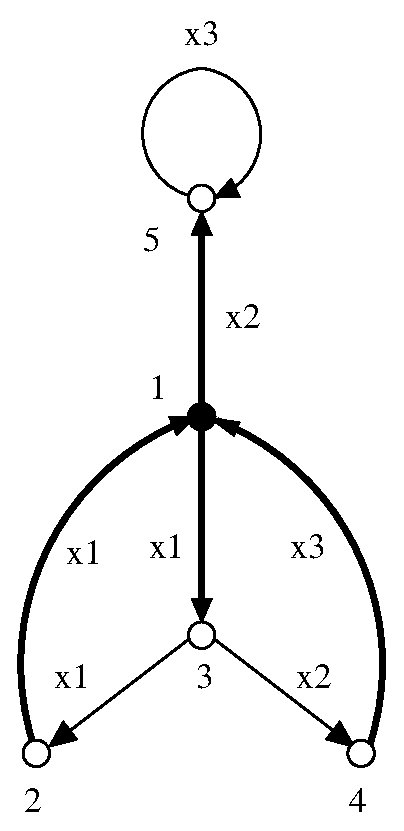
\includegraphics[scale=.5]{stallh1.eps}
\label{fig:stall1} } \hspace{15mm} \subfigure[Stallings automaton
for $H_2$.]{
A pic called stallh2
%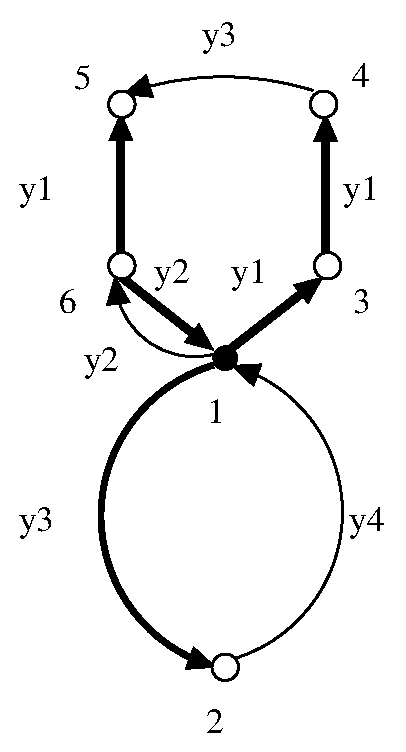
\includegraphics[scale=.5]{stallh2.eps}
\label{fig:stall2} }
\end{center}
\caption{Stallings automata for subgroups $H_1,
H_2$}\label{fig:stall}
\end{figure}

Systems of inner representatives (corresponding to the choice of
maximal subtrees) of $H_1$ in and $H_2$ in $F_2$
 are $S_{1,in} = \{1,x_1,x_1^{-1},x_2,x_3^{-1} \}$ and $S_{2,in} = \{1, y_1, y_1^2,
y_2^{-1}, y_2^{-1}y_1, y_3 \}$.

We want to find double coset normal form for elements $f_1 =
x_2x_3^2x_2^{-1} x_1^4x_3^3x_1^{-2}x_3^{-1}x_2^{-1}x_1^{-1}$ and
$f_2=y_1^2y_3y_1^{-1}y_2y_3y_4y_1y_2 y_3y_4y_2^2$.

Consider the element $f_1 \in F_1$ first.

\begin{align*}
f_1 &= (h_2^2h_1)\cdot x_1x_3^3x_1^{-2}x_3^{-1}x_2^{-1}x_1^{-1} =
(h_2^2h_1)\cdot x_1x_3^3x_1^{-2}\cdot(h_3^{-1})\\
&= (h_2^2h_1)\cdot x_1 \circ x_3^3x_1^{-1}\circ
x_1^{-1}\cdot(h_3^{-1})
\end{align*}

To rewrite $f_2$ in normal form, we need to describe
representatives of type $2$ in this case. Namely, $(y_1^2,
y_2^{-1}y_1) \sim (y_1,y_2^{-1})$, and since $(y_1,y_2^{-1})$ is
minimal one, then we chose it to be representative of equivalence
class $\pp = \{(y_1,y_2^{-1})(y_1^2, y_2^{-1}y_1),  \}$. Further,

\begin{align*}
f_2 &= y_1^2y_3y_1^{-1}y_2y_3y_4y_1y_2y_3y_4y_2^2\\ &=
((h_3^{\prime})^2h_2^{\prime}) \cdot y_1 \circ (y_2^{-1})^{-1}
\cdot(h_2^{\prime}h_1{\prime})=
\end{align*}


\end{example}

%%
%%
%%As before let $g$ be a word in $F_1\ast F_2$ and suppose that
%%$g=g_1\cdots g_t$ in reduced form. Denote $S= S_1 \cup S_2$, where
%%$S_1$ are sets of double coset representatives for $H_1$ and $H_2$
%%correspondingly. Write each syllable $g_i$ of $g=g_1\cdots g_t$ in
%%normal form using the algorithm above. This gives
%%$g_i=h_{i,1}d_ih_{i,2}$, with $d_i\in S$ and $h_{i,j}\in H_1\cup
%%H_2$. Using $\phi_1^{-1}$ or $\phi_2^{-1}$, as appropriate, we now
%%write $h_{i,1}$ and $h_{i,2}$ as reduced words in $F(Z)$. For
%%$i=1,\ldots , t-1$, we reduce the word $h_{i,2}h_{(i+1),1}\in
%%F(Z)$ to give a reduced word $h_i\in F(Z)$ and set $h_0=h_{1,1}$
%%and  $h_{t+1}=h_{t,2}$. Then $g$ has normal form $h_0d_1h_1\cdots
%%d_th_{t+1}$.
%%
%%
%%\begin{example}\label{ex:g}
%%Let $g =f_1 f_2 f_1^{-1}$ in settings of Example \ref{ex:f_1f_2}.
%%Set $z_i = h_i = h_i^{\prime}$ for $i= 1,2,3$; then
%%
%%\begin{align*}
%%g &= (z_2^2z_1)\cdot x_1 \circ x_3^3x_1^{-1} \circ x_1^{-1}\cdot
%%(z_3^{-1}z_3^2z_2) \cdot y_1 \circ (y_2^{-1})^{-1}\\ &\cdot(z_2 z_1 z_3)\cdot x_1\circ x_1 x_3^{-3} \circ x_1^{-1}\cdot (z_1^{-1}z_2^{-2})=\\
%%&(z_2^2z_1)\cdot d_1(x) \cdot (z_3z_2) \cdot d_2(y) \cdot(z_2 z_1
%%z_3) \cdot d_1(x)^{-1} (z_1^{-1}z_2^{-2}).
%%\end{align*}
%%
%%
%%
%%\end{example}

%
%%%
%
%%%%%%%%%%%%%%%%%%%%%%%%%%%%%%%%%%%%%%%%%%%%%%%%%
\section{The generalised folding process}\label{sec:foldings}
The object is to construct an automaton which will accept a word $w$
in double coset normal form if and only if it belongs to a given subgroup $K$.
The idea is to this by starting with the flower automaton for the
generators of $K$, written in (double coset) normal form; carrying out
Stallings folding as usual to produce a deterministic, trim, inversive
automaton; and next adding some additional paths to allow normal forms
to be read. This may introduce new non-determinism in some  states (i.e. edges
which may be folded), so
the resulting automaton must be folded again.
The result of the final folding is the candidate automaton.

 Suppose $L$ is the
language accepted by the flower automaton of $K$. The image of $L$ under
the canonical map to $G$ is $K$. All the stages of our generalised folding
process will preserve this image, so our final automaton will accept a language
$L_1$ which also maps to $K$. We must then prove that if $w$ is a word
in normal form which represents an element of $K$ then $w$ is in $L_1$. It will
therefore suffice to show that if $u$ is any word in $L_1$ then the
normal form of $u$ is also in $L_1$.

Recall from above that we have $F_1$, $F_2$ free groups (finitely
generated by $X_1$ and $X_2$, respectively);
 $H_1 \leq F_1$, $H_2 \leq F_2$ such that
there exists an isomorphism $\phi: H_1 \rightarrow H_2$; a free group
 $F(Z)$, generated by $Z=\{z_1, \ldots, z_m\}$,
and  maps $\phi_1$ and $\phi_2$ such that $\phi_1(z_i)=h_i(X_1)  $
and  $\phi_2(z_i)=h^\prime_i(X_2)$, $i=1,\ldots ,m$, both of which
induce isomorphisms with $\phi=\phi_2\phi_1^{-1}$. Implicit in all
this is that $X_1\cap X_2=X_1\cap Z = X_2\cap Z=\nul$. We define
${G = F_1 \underset{H_1=H_2}{\ast} F_2}$, the group with
 presentation $\la X_1,X_2 | h_i = h_i', i=1 \ldots m\ra$ and
let $S_1$ and $S_2$ be sets of  double coset representatives of
$H_1\le F_1$ and $H_2\le F_2$, respectively, (as in Section
\ref{sec:intro}); denote $S= S_1 \cup S_2$. Let $A_k$ be the
Stallings automaton for $H_k$ and let $T_k$ be a spanning tree for
the associated graph $\G_{A_k}$, $k=1,2$.

%\subsection{Construction of the double coset normal form}\label{sub:construction_dcnf}}
Suppose that $g \in G$ and $g=g_1\cdots g_t$ is in reduced form.
Write each syllable $g_i$ of $g=g_1\cdots g_t$ in normal form
using the algorithm I above. This gives
$g_i=h_{i,1}d_ih_{i,2}$, with $d_i\in S$ and $h_{i,j}\in H_1\cup
H_2$. Using $\phi_1^{-1}$ or $\phi_2^{-1}$, as appropriate, we now
write $h_{i,1}$ and $h_{i,2}$ as reduced words in $F(Z)$. For
$i=1,\ldots , t-1$, we reduce the word $h_{i,2}h_{(i+1),1}\in
F(Z)$ to give a reduced word $h_i\in F(Z)$ and set $h_0=h_{1,1}$
and  $h_{t+1}=h_{t,2}$. Then $g$ has normal form $h_0d_1h_1\cdots
d_th_{t+1}$.


\begin{example}\label{ex:g}
Let $g =f_1 f_2 f_1^{-1}$ in settings of Example \ref{ex:f_1f_2}.
Set $z_i = h_i = h_i^{\prime}$ for $i= 1,2,3$; then

\begin{align*}
g &= (z_2^2z_1)\cdot x_1 \circ x_3^3x_1^{-1} \circ x_1^{-1}\cdot
(z_3^{-1}z_3^2z_2) \cdot y_1 \circ (y_2^{-1})^{-1}\\ &\cdot(z_2 z_1 z_3)\cdot x_1\circ x_1 x_3^{-3} \circ x_1^{-1}\cdot (z_1^{-1}z_2^{-2})=\\
&(z_2^2z_1)\cdot d_1(x) \cdot (z_3z_2) \cdot d_2(y) \cdot(z_2 z_1
z_3) \cdot d_1(x)^{-1} (z_1^{-1}z_2^{-2}).
\end{align*}

\end{example}


Let $K=\la k_1, \ldots , k_s\ra$, where $k_i$ is an element of $G$
written in normal form: say
\begin{equation}\label{eq:k-form}
k_i= h_{i,0}t_{i,1}h_{i,1}\cdots t_{i,m_i}h_{i,m_i+1},
\end{equation}
where $h_{i,j}\in F(Z)$ and $t_{i,j}\in S_1\cup S_2$.

\subsection{Double coset automata and graphs}
\begin{comment}
A colouring of a directed, inversive, labelled graph $\G$ is a map $c$  from $V(\G)\cup E(\G)$
 to a set $C$ such that if $\i_E$ is the involution on edges
then $c(e)=c(\i(e))$. (We make no conditions on the colouring of
vertices: in particular adjacent vertices may have the same
colour.)

\begin{definition}
A finite, rooted, directed, labelled, coloured graph $\G$ is called a
{\em double-coset-graph} or
{\em dc-graph}
if $\G$ has vertices, edges, labelling function and colouring function,
 $V$, $E$, $l$ and $c$,
respectively, satisfying the following conditions.
\be[(i)]
\item $l$ is a map $l:E\maps X_1\cup X_2\cup Z$.
\item $c$ is a map $c:V\cup E\maps \ZZ\times \ZZ$.
\item $E=E_Z\cup E_{X_1}\cup E_{X_2}$,
where $E_Z=l^{-1}(Z)$, $E_{X_1}=l^{-1}(X_1)$ and $E_{X_2}=l^{-1}(X_2)$.
\item $V=V_0\cup V_C$, where $V_0=V\bs V_C$ and
$V_C$ is the union of
$V_{X_1}$, $V_{X_2}$ and $V_Z$, with
$V_Y=\{\textrm{vertices incident only to edges of } E_Y\}$, for $Y=Z,X_1$ or $X_2$.
\item Let $c_k:V\cup E\maps \ZZ$ be the composition of $c$ with projection
onto the $k$th factor of $\ZZ\times \ZZ$, for $k=1$ or $2$. Then
$c_k(x)\ge 0$, for all $x\in V\cup E$ and  for $k=1$ and $2$.
\item   For all $v\in V$,
$c_1(v)+c_2(v)>0$ if and only if $v\in V_0$. Moreover, if $v\in V_0$ then
$c_k(v)=\max\{c_k(e): e \textrm{ is incident to } v\}$.
\ee
An automaton $A$ is called a {\em dc-automaton} if $\G_A$ is  a dc-graph.

\end{definition}


\begin{example}\label{ex:dc-graph}
Figure \ref{fig:dc-grapha} shows a dc-graph, with root $\a$,
where $x\in X_1$, $y_1,y_2,y_3\in X_2$,
$z\in Z$, the only vertex not in $V_0$ is $\d$,
colours of all edges are shown and the colours of vertices  are
$c(\a)=(3,0)$, $c(\b)=(3,0)$, $c(\g)=(0,2)$, $c(\d)=(0,0)$, $c(\e)=(0,2)$ and
$c(\z)=(1,0)$.
\end{example}
\begin{figure}
\begin{center}
\psfrag{a}{$\a$}
\psfrag{b}{$\b$}
\psfrag{c}{$\g$}
\psfrag{d}{$\d$}
\psfrag{e}{$\e$}
\psfrag{f}{$\z$}
\psfrag{g}{$\eta$}
\psfrag{h}{$\theta$}
\psfrag{x}{$x$}
\psfrag{z}{$z$}
\psfrag{y1}{$y_1$}
\psfrag{y2}{$y_2$}
\psfrag{y3}{$y_3$}
\psfrag{(1,0)}{$(1,0)$}
\psfrag{(0,0)}{$(0,0)$}
\psfrag{(0,2)}{$(0,2)$}
\psfrag{(3,0)}{$(3,0)$}
\subfigure[A dc-graph...]{
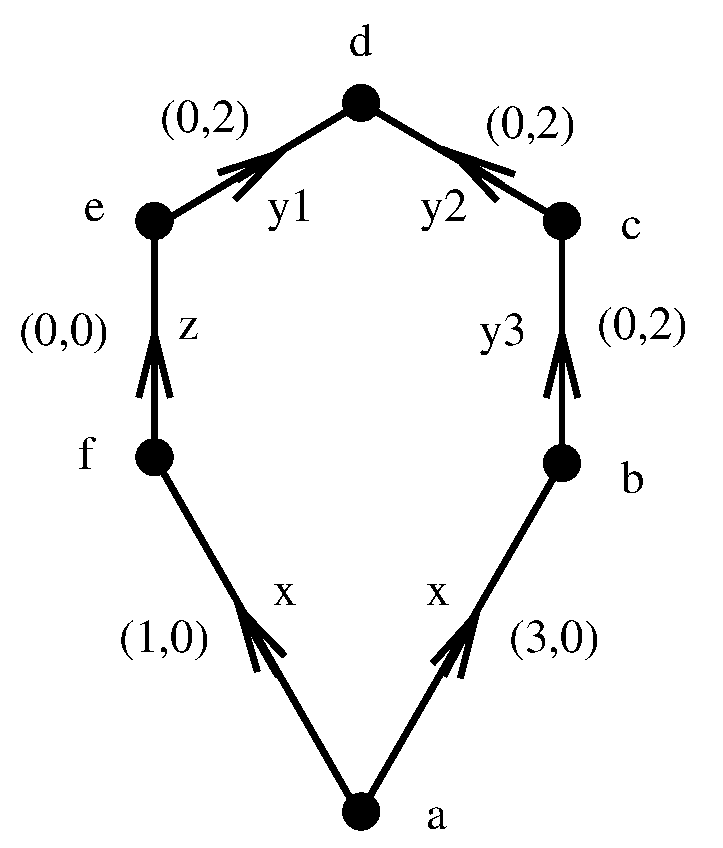
\includegraphics[scale=.5]{dc-graph.eps}
\label{fig:dc-grapha}
}
\hspace{15mm}
\subfigure[... and its Stallings folding]{
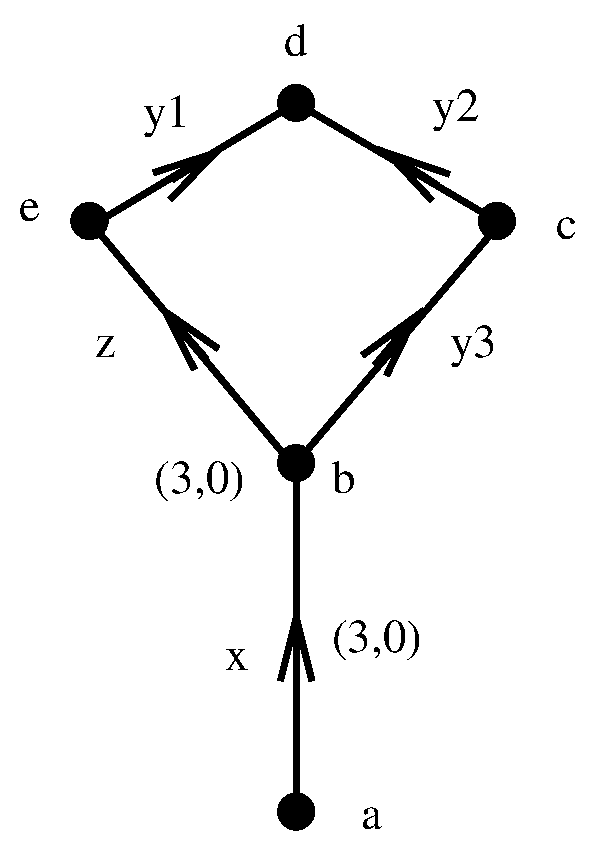
\includegraphics[scale=.5]{dc-folded.eps}
\label{fig:dc-graphb}
}
\end{center}
\caption{Folding a  dc-graph}\label{fig:dc-graph}
\end{figure}
An {\em elementary dc-folding} of a dc-graph $\G$ is a graph $\G^\prime$
obtained from $\G$ as follows. Suppose that $e=(p,a,q)$ and
$e^\prime=(p,a,q^\prime)$
are edges of $\G$. (We do not require $p$, $q$ and $q^\prime$ to be distinct.)
% with $c(p)=(m_1,n_1)$, $c(q)=(m_2,n_2)$,
%$c(q^\prime)=(m_3,n_3)$, $c(e)=(r_1,s_1)$ and $c(e^\prime)=(r_2,s_2)$.
 Then $\G^\prime$ is the quotient of $\G$ formed by identifying
$q$ and $q^\prime$, to form a new vertex $q^{\prime\prime}$; and
$e$ and $e^\prime$, to form a new edge
$e^{\prime\prime}=(p,a,q^{\prime\prime})$. If the root of $\G$ is $q$
 or $q^\prime$ then $q^{\prime\prime}$ is the root of $\G^\prime$ and otherwise
 the root of $\G^\prime$ is that of $\G$. The colouring
  map of $\G^\prime$
is the same as that of $\G$ except that
 $c_k(\e^{\prime\prime})=\max\{c_k(e),c_k(e^{\prime\prime})\}$
and $c_k(q^{\prime\prime})=\max\{c_k(q),c_k(q^{\prime\prime})\}$,
for $k=1,2$. {\ef
$c_k(e^{\prime\prime})=\max\{c_k(e),c_k(e^{\prime})\}$ and
$c_k(q^{\prime\prime})=\max\{c_k(q),c_k(q^{\prime})\}$ ?} From the
definition, the conditions for a dc-graph are satisfied by
$\G^\prime$. A {\em dc-folding} of a dc-graph $\G$ is a graph
obtained from $\G$ by a finite sequence of elementary foldings.
Thus a dc-folding of a dc-graph is again a dc-graph.

From now on we shall assume, unless we explicitly indicate otherwise,
 that all graphs are dc-graphs and  all foldings are dc-foldings.
\end{comment}

An {\em elementary folding} of a graph $\G$ is a graph $\G^\prime$
obtained from $\G$ as follows. Suppose that $e=(p,a,q)$ and
$e^\prime=(p,a,q^\prime)$
are edges of $\G$. (We do not require $p$, $q$ and $q^\prime$ to be distinct.)
 Then $\G^\prime$ is the quotient of $\G$ formed by identifying
$q$ and $q^\prime$, to form a new vertex $q^{\prime\prime}$; and
$e$ and $e^\prime$, to form a new edge
$e^{\prime\prime}=(p,a,q^{\prime\prime})$. If the root of $\G$ is $q$
 or $q^\prime$ then $q^{\prime\prime}$ is the root of $\G^\prime$ and otherwise
 the root of $\G^\prime$ is that of $\G$.
 A {\em folding} of a graph $\G$ is a graph obtained
from $\G$ by a finite sequence of elementary foldings.

A graph on which  it is not possible to perform an elementary
folding is
said to be {\em folded}. A {\em Stallings folding} of a graph $\G$ is
 a (possibly trivial) folding of $\G$ which is folded. As every non-trivial
folding decreases
 the number of edges of the graph, every graph has a Stallings folding.
From the
standard theory (e.g. Enric's notes \cite{ventura11}) a Stallings folding of a graph is unique,
so we may define {\em the Stallings folding} $S(\G)$ of a graph $\G$.
\begin{comment}
~\\
({\bf This is not quite clear, because it needs to be established
that colouring of a Stallings folding of $\G$ is not dependent on
the order of folding. It would be enough to show that the morphism
from $\G$ to $S(\G)$ is uniquely determined by $\G$, but I haven't
checked this out.}{\ef It seems to be true, but I didn't check it
out properly yet.})
\begin{example}
Figure \ref{fig:dc-graphb} shows the Stallings folding of the graph of
Example \ref{ex:dc-graph}. Colours are shown only where the folding changes them.
\end{example}
%
%
\end{comment}

Now let $\cF(K)$ be the flower automaton of $K$ and let
$\G$ be the corresponding rooted graph. If $e$ is an edge of $\G$ then
$e$ is labelled by a letter (of $X_1\cup X_2 \cup Z$)
occuring in $h_{i,j}$ or $t_{i,j}$, for some $i,j$, as in
\eqref{eq:k-form}. If $e$ is labelled by a letter of $Z$ we say $e$ has {\em type} $Z$.
 %and define $c(e)=(0,0)$.
If $e$ is labelled by a letter of $X_k$ occuring in
$t_{i,j}$, we say $e$ has {\em type} $X_k$.
\begin{comment}
 and define
\[c_k(e)=m_1+\cdots m_{i-1} +j\textrm{ and } c_{k^\prime}(e)=0,\]
where $k\neq k^\prime$. If $v\in V_C$ then we define $c(v)=(0,0)$. If $v\in V_0$ then
 we define $c_k(v)=\max\{c_k(e): e \textrm{ is incident to } v\}$, for $k=1,2$.
This makes $\G$ into a dc-graph. The graph of Example \ref{ex:dc-graph} is obtained
from the subgroup $K$ generated by the single element $xzy_1y_2y_3x^{-1}$ in this way.
\end{comment}

Now let $\D$ be the Stallings folding of the graph $\G$.  Then
 $\D$ is a connected, deterministic, trim, graph and $\pi(L(\D))=K$. However
$L(\D)$ does not, in general, contain all normal forms of elements of $K$.
Next we transform $\D$ to allow it to accept normal forms.

\begin{comment}
\begin{definition}\label{def:attractive}
Let $\D$ be a  dc-graph, let $k\in \{1,2\}$ and let
$u,v\in V_0(\D)$ such that
\be[(i)]
\item $c_k(u)\neq c_k(v)$ and
\item there exists a path $p$ from $u$ to $v$ in $\D$ with label $l(p)$
a word in $F(X_k\cup Z)$.
\ee
Then the pair $(u,v)$ is said to be
$k${\em -attracting} with {\em link} $p$ and {\em resolution}
$r(u,v)$ the normal
form of $l(p)$ in $F(X_k)$.
\end{definition}

We set
\begin{align}
A_k&=\{\{u,v\}\subseteq V_0(\D): (u,v) \textrm{ is an attracting pair}\} \textrm{ and }\\\label{eq:attset}
\vec{A_k}&=\{(u,v)\in V_0\times V_0: \{u,v\}\in A_k\}.
\end{align}
As a direct consequence of the definitions we have the following lemma.
\begin{lemma}
If $\{u,v\}$ and $\{v,w\}\in A_k$ and $c_k(u)\neq c_k(v)$ then
$\{u,w\}\in A_k$.
\end{lemma}
\end{comment}



Let $\D_k$ be the graph formed from $\D$ by removing all edges of
type $X_{k^\prime}$, where $k\neq k^\prime$. An $X_k$ component of
$\D_k$ is the subgraph of $\D$ formed from a connected component
of $\D_k$ by removing all leaves which are incident to edges of
type $Z$, and then repeating the process till there are no such
leaves left.
 We shall modify the $X_k$ components of $\D_k$ so that normal forms of words
are readable.

Let $\T$ be an $X_k$ component of $\D_k$. A
{\em boundary vertex} of $\T$ is defined to be a vertex
$\a$ such that $\a$ is incident, in $\D$, to a vertex which does not
belong to $\T$.  If $(\a,z,\b)$ is an edge of
$\T$ labelled by an element $z\in Z$ then add a path from $\a$ to
$\b$ labelled by $\phi_k(z)$ to the graph $\T$. Do this for all such edges
and call the result $\T_1$.  Define the boundary vertices of $\T_1$ to be
the boundary vertices of the subgraph $\T$. Similarly, the images of these
boundary vertices are defined to be the boundary vertices of
the graphs $\T_2$, $\T_3$, $\T_4$ and $\T_5$ constructed
below.

Given labelled graphs $\G_1$ and $\G_2$ we define the {\em
product} graph $\G_1\times \G_2$ to be the graph with vertices
$V=V(\G_1)\times V(\G_2)$ and with a directed edge labelled $a$
from $(u_1,u_2)$ to $(v_1,v_2)$ if and only if there are edges
$(u_1,a, v_1)$ and $(u_2,a,v_2)$ in $\G_1$ and $\G_2$,
respectively. Let $\cP=\T_1\times \G_{A_k}$. Then there is a path
 labelled $w$ from $\a$ to $\b$
in $T_1$ {\ef {$\T_1$?}}and a path labelled $w$ from $\a^\prime $
to $\b^\prime$ in $\G_{A_k}$ if and only if there is a path
labelled $w$ from $(\a,\a^\prime)$ to $(\b,\b^\prime)$ in $\cP$.
 We shall
use this property of $\cP$ to determine which new paths to add  to $\T_1$.
Choose a spanning  subtree $\U$ of  $\cP$. Next
 order the vertices of
$\T_1$: say these are $\a_0,\ldots, \a_t$, in the order written.

Let $\a_i$, $\a_j$ be vertices of  $\T_1$ with $i\le j$. If there
exists a simple path $p$ in $\cP$ from $(\a_i,1)$ to $(\a_j,1)$
then let $l_p\in F(X_k)$ be the label of $p$ and let
$w_p=\phi_k^{-1}(l_p)\in F(Z)$. Let $q$ be a path (disjoint from
$\T_1$) of length $|w_p|$ and with label $w_p$. Identify the
initial vertex of $q$ with $\a_i$ and the terminal vertex of $q$
with $\a_j$. Now fold the resulting graph. Repeat this process for
all simple paths from  $(\a_i,1)$ to $(\a_j,1)$, over all pairs of
vertices $\a_i$, $\a_j$ with $i\le j$. Call the resulting graph
$\T_2$. There are finitely many simple paths in $\cP$ so this
process terminates. Moreover, regarding $\T_1$ and $\T_2$ as
automata, if $\a$ and
 $\b$ are
boundary vertices of $\T_1$ and $L_1$ and $L_2$ are the
languages accepted by $(\T_1,(X_k\cup Z), \a,\b)$ and
$(\T_2,(X_k\cup Z), \a,\b)$, respectively, then $\pi(L_1)=\pi(L_2)\subseteq G$.

As the edges added to $\T_1$ to form $\T_2$ are all labelled by elements
of $Z$, and all edges of $\G_{A_k}$ are labelled by elements of $X_k$
the graphs $\cP=\T_1\times \G_{A_k}$ and $\T_2\times \G_{A_k}$ differ only
in that the second may have some new isolated vertices. For our purposes
we may discard these and assume that $\cP=\T_1\times \G_{A_k}=
 \T_2\times \G_{A_k}$. If $\cP=\U$ then we have nothing to do at the
next stage and we immediately set $\T_3=\T_2$. Otherwise,
suppose that $e$ is an edge of $\cP$ which does not belong to $\U$ but
which does belong to a component $\Xi$  of $\cP$ containing a vertex
$(\a,1)$, for some vertex $\a$ of $\T_2$.
Let $(\a,1)$ be such a vertex and let
$e=((\a_i,\b_1), x, (\a_j,\b_2))$,
 with label $x\in X_k$.
%Let
%$\a_m$ be the minimal vertex of $\T_2$ (necessarily also a vertex
%of $\T_1$)  such that $(\a_m,1)$ belongs to $\Xi$.
 Let $p_i$ be
the path in $\U$ from $(\a,1)$ to $(\a_i,\b_1)$ and let $p_j$ be
the path in $\U$ from  $(\a_j,\b_2)$ to $(\a,1)$ and
let $l_i$ and $l_j$ be the labels of $p_i$ and $p_j$, respectively. Then
$p_i,e,p_j$ projects to a closed path in $\G_{A_k}$, based at $1$, with
label $h_e=l_i x l_j \in H_k\subseteq F_k$. Moreover
$p_i,e,p_j$ projects to a closed path in $\T_2$, based at $\a$, also
with label $h_e$. Let
$w_e=\phi_k^{-1}(h_e)$ and let
$q$ be a path (disjoint from $\T_2$) of length
$|w_e|$ and with label $w_e$. Identify the initial and terminal
vertices of $q$ to $\a_i$ and $\a_j$, respectively, and fold the
resulting graph. Repeat this process for all such edges $e$ and
vertices $(\a,1)$ of $\cP$
and denote the result by $\T_3$.
(In practice it's not necessary to
repeat this process for {\em all} such vertices $(\a,1)$ in $\Xi$: but it
makes the proofs later easier if we assume that we do so.)
If
$L_3$ is the
language accepted by $(\T_3,(X_k\cup Z), \a,\b)$, for boundary
vertices $\a$, $\b$ of $\T_1$, then again $\pi(L_3)=\pi(L_1)$.


Next we wish to add paths to $\T_3$ that allow us to read the normal
forms of words $w$ which are readable by $\T_3$ and readable,
but not accepted, by $\G_{A_k}$.
As before we may assume that
$\cP=\T_1\times \G_{A_k}=
 \T_3\times \G_{A_k}$.
Recall that we have fixed a spanning subtree
$T_k$ of $\G_{A_k}$.
Let $\d=(\a_j,\b)$ be a vertex of $\cP$, with $\b\neq 1$, which lies
in a connected component of $\cP$ containing a vertex  $\g=(\a_i,1)$,
for some vertex $\a_i$ of $\T_3$.
Let $b$ be the label of the path in $T_k$ from $1$ to $\b$.
 If $\cP$ contains a simple
path from $(\a_i,1)$ to $(\a_j,\b)$, with label $b$,  then
 say that $\cP$ {\em covers} the pair $\g,\d$.
If all such pairs of vertices are covered by $\cP$ then set $\T_4=\T_3$.
Otherwise
let $p$ be the simple path in $\U$ from a
vertex $\g=(\a_i,1)$ to a vertex $\d=(\a_j,\b)$, where $\g,\d$
is not covered by $\cP$.
 Let
$p$ have label $a$.
Then $ab^{-1}=h\in H_k$. Let
$w=\phi_{k}^{-1}(ab^{-1})
\in F(Z)$ and let $q$ be a path (disjoint from $\T_3$)
with label $wb$. Identify the initial
and terminal vertices of $q$ with vertices $\a_i$ and $\a_j$ of $\T_3$,
respectively, and fold
the resulting graph.
As $\pi(a)=\pi(wb)\in G$ the image of the language accepted by
the resulting graph (considered as an automaton with start state  $\a_i$
 and final
state $\a_j$) is unchanged by
this operation.
Repeat this process for all pairs of  vertices which are not
covered by $\cP$ and
call the result $\T_4$.

Finally we wish to add paths which allow double coset representatives
of type $2$ to be read. Suppose $(\e,\xi)\in \G_{A_k}\times \G_{A_k}$ and
that the $\sim$ representative of $(\e,\xi)$ is $(\e_0,\xi_0)$.
Let $b_1$ and $b_2$ be the labels
of paths $w(\e)$ and $w(\xi)$, from $1$ to $\e$ and $1$ to $\xi$ in the
subtree $T_k$ of $\G_{A_k}$. Let $a_1$ and $a_2$ be the labels of
paths $w(\e_0)$ and $w(\xi_0)$. Then there are  paths in $\G_{A_k}$,
with label
$c=c(\e,\xi)$, from $\e$ to $\e_0$ and from $\xi$ to $\xi_0$.
Furthermore $h_i=
b_ica_i^{-1}\in H_k$ and $w_i=\phi_k^{-1}(h_i)\in F(Z)$, for $i=1,2$.
If there
exist paths $p_1$, with label $b_1$ from $(\a_i,1)$ to $(\a_j,\e)$,
and $p_2$, with label $b_2$ from
$(\a_l,1)$ to $(\a_j,\xi)$, in $\U$,  then
let $q$ be a path (disjoint from $\T_4$)
with label $w_1 a_1a_2^{-1} w_2^{-1}$,
and identify the initial
and terminal vertices of $q$ with  vertices $\a_i$ and $\a_l$
of $\T_4$, respectively.
Fold the resulting graph.
To see that the image of the language accepted by
 the new graph is the same as that of the original note
that the word $b_1b_2^{-1}$ is readable, starting at $\a_j$ and
ending at $\a_l$, in $\T_4$. As $\pi(b_1b_2^{-1})=\pi(w_1a_1a_2^{-1}w_2^{-1})$
the addition of this new path has no effect on the image, under $\pi$, of
the language accepted.
%$d_1$ and
%$d_2$ be labels of paths $p_1$ and $p_2$ in $\cP$ and let $e_1$ and
%$e_2$ be labels of simple paths with the same end points. Then
%$d_ie_i^{-1}\in H_k$ and  there is a path
%in $\T_4$ with label $\phi_k(d_ie_i^{-1})e_i$, for $i=1,2$. Moreover,
%$\T_4$ contains a path
%with label $\phi_k(e_ib_i^{-1})b_i$ and so a path with label
%$\phi(d_ib_i^{-1})b_i$, $i=1,2$.
Repeat this process for all such paths $p_i$ and $p_j$ and all such
pairs $(\e,\xi)$ to form $\T_5$.

\begin{lemma}
Let $\a$ and $\b$ be boundary vertices of $\T_1$ and let $w$ be a word
 which is accepted by the automaton $(\T_1, X_k\cup Z, \a, \b)$. Then the
normal form of $w$ is accepted by $(\T_5, X_k\cup Z, \a, \b)$.
\end{lemma}
\begin{proof}
We may assume that $w\in F(X_k)$ (given the construction of $\T_1$).
Let $w$ have normal form $h_1s h_2$, where $s\in S_k$ and $h_i\in F(Z)$.
There are two cases to consider, depending on whether $s$ is a
representative of type $1$ or type $2$.
 First consider the case where $s$ is of type $1$, say
 $s= a_1 c a_2^{-1}$, where
$a_1$ and $a_2$ are labels
of simple paths in the subtree $T_k$, $c$ is non-empty
and $c$ and $c^{-1}$ have
no non-trivial prefix which is readable in $A_k$. Then there are words
$g_1, g_2, b_1$ and $b_2\in F(X_k)$ such that
$w=g_1\circ b_1\circ c \circ b_2^{-1}\circ g_2^{-1}$,
$g_i\in H_k$, $b_i$ is readable but not accepted by  $A_k$ and
$\phi_k(h_i)=g_ib_ia_i^{-1}$, $i=1,2$.

Since $g_i\in H_k$ and $w$ is accepted by $\T_1$ there is a path
labelled $g_1$ from $\a$ to a vertex $\a_1$ of $\T_1$ and a path
labelled $g_2$ from $\b$ to a vertex $\a_2$ of $\T_1$. Therefore, in $\cP$,
there are paths $p_1$ from $(\a,1)$ to $(\a_1,1)$ labelled $g_1$, and
$p_2$
from $(\b,1)$ to $(\a_2,1)$ labelled $g_2$.
Now $p_1$ may
be written as a concatenation of paths $p_1=o_0e_1\cdots e_l o_{l}$,
where $o_i$ is a simple path in $\U$ and $e_i$ is an edge of $\cP$ which does
not belong to $\U$.  Let $e_i$ have initial and terminal vertices
$\g_i$ and $\d_i$ and let $L_i$ and $R_i$ be the simple paths in $\U$ from
$(\a,1)$ to $\g_i$ and from $\d_i$ to $(\a,1)$, respectively.
Then, for $i=1,\ldots ,l$,
the path $L_i e_i R_i$ is a closed path in $\cP$, based
at $(\a,1)$, containing exactly one edge, $e_i$, which is not in $\U$.
Thus the label of  $L_i e_i R_i$ is $h_i\in H_k$ and $\phi_k^{-1}(h_i)$ is the
label of a closed path in $\T_3$, based at  $\a$. (All such paths
were added in the construction of $\T_3$ from $\T_2$.)
Also, there is a path $q_1$ in $\U$ from $(\a,1)$ to $(\a_1,1)$, with
label $h_{l+1}$, and by construction of $\T_2$ there is a path from $\a$ to
$\a_1$ in $\T_2$ with label $\phi_k^{-1}(h_{l+1})$.
The path
$p_1$ is the result of reducing (deleting adjacent edges $e,e^{-1}$) the path
$o_0 e_1 (R_1 R_1^{-1}) o_1 \cdots e_{l}(R_l R_l^{-1}) o_{l}$.
Moreover $o_0=L_1$; for $2\le i\le l$,
$L_i$ is the path obtained by reducing $R_{i-1}^{-1}o_{i-1}$; and
$R_{l}^{-1}o_{l}$ reduces to the path in $\U$ from
$(\a,1)$ to $(\a_1,1)$, that is to $q_1$.
Since the
order in which these reductions are carried out does not affect the end
result we may regard $p$ as the result of reducing the path
$L_1 e_1 R_1 \cdots L_l e_l R_l q_1$. Hence the label $g_1$
of $p_1$ is the result of
reducing the word $h_1\cdots h_l h_{l+1}$ and $\phi_k^{-1}(g_1)$ is the result of
reducing $\phi_k^{-1}(h_1) \cdots \phi_k^{-1}(h_{l+1})$. As each $\phi_k^{-1}(h_i)$ is readable
in $\T_3$ and $\T_3$ is folded this means  that $\phi_k^{-1}(g_1)$ is the
label of a path, from $\a$ to   $\a_1$, in $\T_3$. Similarly,
$\phi_k^{-1}(g_2)$
is the label of a path from $\b$ to $\a_2$ in $\T_3$.

The word $b_1$ is readable by $\G_{A_k}$ and there
is a path with label $b_1$ in $\T_1$ from $\a_1$ to some vertex $\b_1$.
Hence $b_1$ is the label of a path in $\cP$ from $(\a_1,1)$ to
$(\b_1,\e_1)$, for some vertex $\e_1$ of $\G_{A_k}$.
By definition $a_1$ is the label of a path in $T_k$ from $1$ to $\e_1$.
Let $b_1^\prime$
 be the label of the simple path $p_1^\prime$ in $\U$ from
$(\a_1,1)$ to $(\b_1,\e_1)$. By construction $\T_4$ contains a path
from $\a_1$ to $\b_1$ with label $h_1^\prime a_1$, where
$h_1^\prime =\phi_k^{-1}(b_1^\prime a_1)\in F(Z)$.
%(and is the empty word if $\cP$ covers $p^\prime$) and
%$b_1^{\prime\prime}$ is the label of the path in $T_k$ from $1$ to
%$\e_1$ (and equals $b_1^\prime$ if $\cP$ covers $p_1^\prime$).
(If $\cP$ covers the pair $(\a_1,1)$, $(\b_1,\e_1)$ then
$b_1^\prime=a_1$ and $h_1^\prime$ is the empty word.)
%Furthermore we have
%$\pi(\phi_k(h_1^\prime)b_1^{\prime\prime})=\pi(b_1^\prime)$.
Now $b_1(b_1^\prime)^{-1}\in H_k$ and is the label of a closed
path  in $\cP$ based at $(\a_1,1)$; so by the
previous part of proof, $\T_3$ contains a closed path, based at $\a_1$,
 with label
$w_1^\prime=\phi_k^{-1}(b_1(b_1^\prime)^{-1})$. Hence, as it is folded,
$\T_4$ contains a path, from $\a$ to $\b_1$,
with label the reduced word obtained from the product
$\phi_k^{-1}(g_1)w_1^{\prime} h_1^\prime a_1$, that is
 $\phi_k^{-1}(g_1b_1a_1^{-1}) a_1=h_1a_1$.
 Similarly, $\T_4$ contains a path from
$\b$ to $\b_2$ with label $h_2a_2$.

As $w$ is the label of a path in $\T_1$ there is a path from $\b_1$ to
$\b_2$ in $\T_4$ with label $c$. Therefore, in this case, $\T_4$ contains
a path from $\a$ to $\b$ which has label the normal form of $w$.

In the second case,
let $w$ have normal form $h_1 a_1 a_2^{-1} h_2^{-1} $, where
$h_1$ and $h_2$ are in $F(Z)$,  $a_1$ and $a_2$ are labels
of simple paths in the subtree $T_k$ and $a_1a_2^{-1}$ is a double coset
representative of type $2$. Then there are words
$g_1, g_2, k_1, k_2, b_1, b_2, c_1$ and $c_2\in F(X_k)$, uniquely
determined by $w$,  such that
$w=g_1\circ b_1 \circ b_2^{-1}\circ g_2^{-1}$,
$g_i, k_i\in H_k$, $b_i$ and $c_i$ are
readable but not accepted by  $A_k$, $c_i$ is the label of
a path in $T_k$, $b_ic_i^{-1}\in H_k$, $a_1a_2^{-1}=k_1c_1c_2^{-1}k_2^{-1}$
 and
$\phi_k(h_i)=g_ib_ic_i^{-1}k_i^{-1}$, $i=1,2$.
As in the first case the word $\phi_k^{-1}(g_1b_1c_1^{-1})c_1 c_2^{-1}
\phi_k^{-1}(c_2b_2^{-1}g_2^{-1})$ is readable in $\T_4$. By construction the
normal form $\phi_k^{-1}(k_1)a_1a_2^{-1}\phi_k^{-1}(k_2^{-1})$ of $c_1 c_2^{-1}$ is readable in
$\T_5$. It follows that the normal form of $w$ is readable in $\T_5$.
\end{proof}


\begin{comment}
Let $d=\max\{c_k(u): u\in V(\T_5)\}$.  For all vertices
in $v\in V_0(\T_5)$ set $c_k(v)=d$ and for all other vertices
of $\T_5$ set $c_k(v)=0$. If $e$ is an edge of  of $\T_5$  of
  type $X_k$ then set $c(e)=(d,0)$.  All other edges of $\T_5$ have
type $Z$ and colour $(0,0)$.
\end{comment}

Replace the subgraph $\T_1$ of $\D$ with $\T_5$, in the obvious
way. Carry through this procedure for each connected component
{\ef Is it so obvious? Components for $k=1$ and $2$ could be not
disjoint(as in example of dc-graph). How to define colour of such
vertices where they intersects?}of $\D_k$, for $k=1$ and $2$. The
resulting graph is said to be obtained from $\D$ by $H$-{\em
resolution}.


\begin{lemma}
Let $\D$ be  a connected, deterministic, trim, graph, let $\T$ be
the graph
obtained from $\D$ by $H$-resolution %of attracting pairs
and let
$\L$ be the Stallings folding of $\T$. Then $\L$ is formed from
$\T$ by folding edges of type $Z$.
\end{lemma}
\begin{proof}
Let $\T=\L_0,\L_1,\ldots, \L_n$ be a sequence of graphs such that
$\L_{i+1}$ is obtained from $\L_i$ by and elementary folding.
Suppose that all these foldings except possibly the last involve only edges
of type $Z$. Assume $L_n$ is formed from $L_{n-1}$ by folding edges
$(\a,x,\b_1)$ and $(\a,x,\b_2)$ with label $x\in X_k$. Since the
first $n-1$ foldings involve only edges of type $Z$ it follows that
if $\g_1$ and $\g_2$ are vertices of $\T$ which map via these foldings
to $\b_1$ and $\b_2$, then there is a path $q$ in $\T$ from $\g_1$ to $\g_2$
which has label in $(Z^{\pm 1}\cup \{x^{\pm 1}\})^\ast$. Hence $\g_1$ and $\g_2$ both belong to
 the same $X_k$ component of $\T$, which also contains the path $q$.
Therefore all $n$ foldings can be carried out in this $X_k$
component. However the $X_k$ components of $\T$ are folded, since they
correspond to the graphs $\T_5$ constructed from $X_k$ components of $\D$.
Therefore no folding involving an edge of type $X_1$ or $X_2$ can occur
in such a sequence, and the result follows.
\end{proof}
\begin{lemma}
Let $\D$ be  a connected, deterministic, trim, graph, let $\T$ be
the graph
obtained from $\D$ by $H$-resolution %of attracting pairs
and let
$\L$ be the Stallings folding of $\T$. Let $\a$  and $\b$ be boundary
vertices of an $X_k$ component of $\L$ and let $p$ be a path from
$\a$ to $\b$ with label $w\in F(X_k\cup Z)$. Then $\L$ contains a
path $q$ with label equal to the normal form of $w$.
\end{lemma}
\begin{proof}
Let $\g$ and $\d$ be vertices of $\T$ which map to $\a$ and $\b$ in the
folding of $\T$ to $\L$. As this folding involves only edges of type $Z$
it follows that $\g$ and $\d$ are in the same $X_k$ component of $\T$.
Moreover there is a path $p^\prime$ in $\T$ such that the image
of $p^\prime$ in $\L$ reduces to $p$. Then $\T$ contains a path
$q^\prime$ such that the label of $q^\prime$ is the normal form of
the label of $p^\prime$. Let $q$ be the reduced path in $\L$ obtained by
reduction of the image of $q^\prime$. Then the images of $l(q)$ and
$l(q^\prime)$ in $G$ are equal and both are equal to the image of $l(p)$ in
$G$. Moreover, since $l(q^\prime)$ is in normal form and $l(q)$ is obtained
from $l(q^\prime)$ by cancellation of letters of $Z$ it follows that
$l(q)$ is in normal form. Hence $l(q)$ is the normal form of $l(p)$,
as required.
\end{proof}
\begin{theorem}
Let $\cA=(\L,X_1\cup X_2\cup Z,\ast)$, where $\L$ is defined in the previous
lemma and $\ast$ is the root of $\L$. Then $\pi(L(\cA))=K$ and if $w$ is the normal form of an element
of $K$ then $w\in L(\cA)$.
\end{theorem}
\begin{proof}
We have $\pi(L(\cA))=\pi(L(\cF(K))=K$, by construction. If $u$ is a word
accepted by $\cA$ then we may write $u=z_0t_1z_1\cdots z_rt_rz_{r+1}$, where
$z_i\in F(Z)$ and $t_i$ is the label of a path between two boundary
vertices of an $X_1$ or $X_2$ component of $\L$, for all $i$. If
$s_i$ is the normal form of $t_i$ then, from the previous lemma, it follows
that $\cA$ also accepts the word $z_0s_1z_1\cdots z_rs_rz_{r+1}$, which
is the normal form of $u$.
\end{proof}
\begin{theorem}
$G$ has solvable subgroup membership problem.
\end{theorem}
%%%%%%%%%%%%%%%%%%%%%%%%%%%%%%%%%%%%%%%%%%%%%%%%%
\bibliographystyle{plain}
\bibliography{membership1}

\medskip



\noindent \textsf{Andrew J. Duncan, School of Mathematics \&
Statistics, Newcastle University, Newcastle upon Tyne, NE1 7RU,
UK}

\noindent {\tt andrew.duncan@ncl.ac.uk}


\noindent \textsf{Elizaveta Frenkel, Moscow State University,
GSP-1, Leninskie gory, 119991, Moscow, Russia}

\noindent {\tt lizzy.frenkel@gmail.com}

\end{document}
